\subsection{Introduction}
Spike trains can be analyzed by exploiting several kinds of techniques, according
to the aim of the analysis. In particular, it might be interesting to study the
behaviour of a recording site after an external stimulation. Notice that this kind
of analysis becomes more and more relevant as it is extended to multiple channels, for
instance in order to study how different neurons react to the same stimulus.
Alternatively, the responses from several subjects can be compared as well. Other
interesting analyses might consist in comparing several channels or corresponding
channels in different subjects, establishing proper metrics to assess similarity
and correlation.

\subsection{Post Stimulus Time Histogram}
Post Stimulus Time Histogram (PSTH) is a vital tool to characterize neural spike trains
in response to a stimulus. Notice that in general the response of a certain neuron
for a repeated given stimulus is not identical, but it tends to change, as in the
adaptation phenomenon.\\
The intensity of the response and its dynamics is visualized through an histogram.
As a matter of fact, a certain time window is isolated after the occurrence of the
stimulus and it is divided into several equally long bins. Then, the total number of
spikes in each bin is counted and reported into the histogram, as shown in the figure
below.
\begin{figure}[H]
    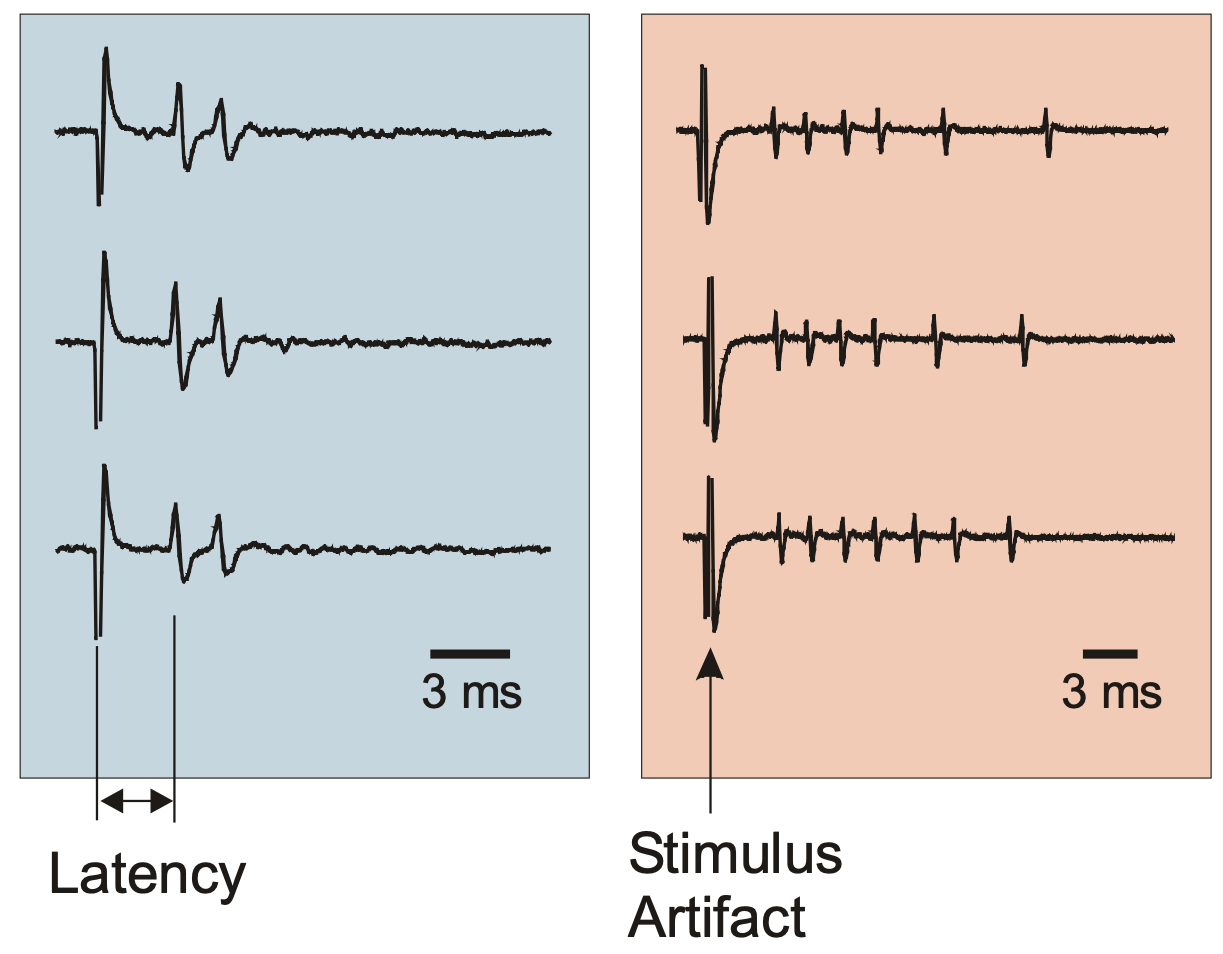
\includegraphics[scale=0.75]{8_1}
    \centering
\end{figure}
Notice that the spike count can be normalized in order to obtain the firing rate, which
can be interpreted also as the probability of firing per time unit.\\
As already state, it is possible to derive several distinct kinds of PSTH, according to
the use case. It can be computed for a single neuron or a single recording site. It
can be computed distinctly for each site of a multi-channel recording, generating
a large number of PST histograms. On the other hand, an averaged PSTH is commonly used
to asses the average response of a network with several recording sites. Nonetheless,
an average PSTH is also employed to consider together spike trains generated in
multiple trials or subjects.
\begin{figure}[H]
    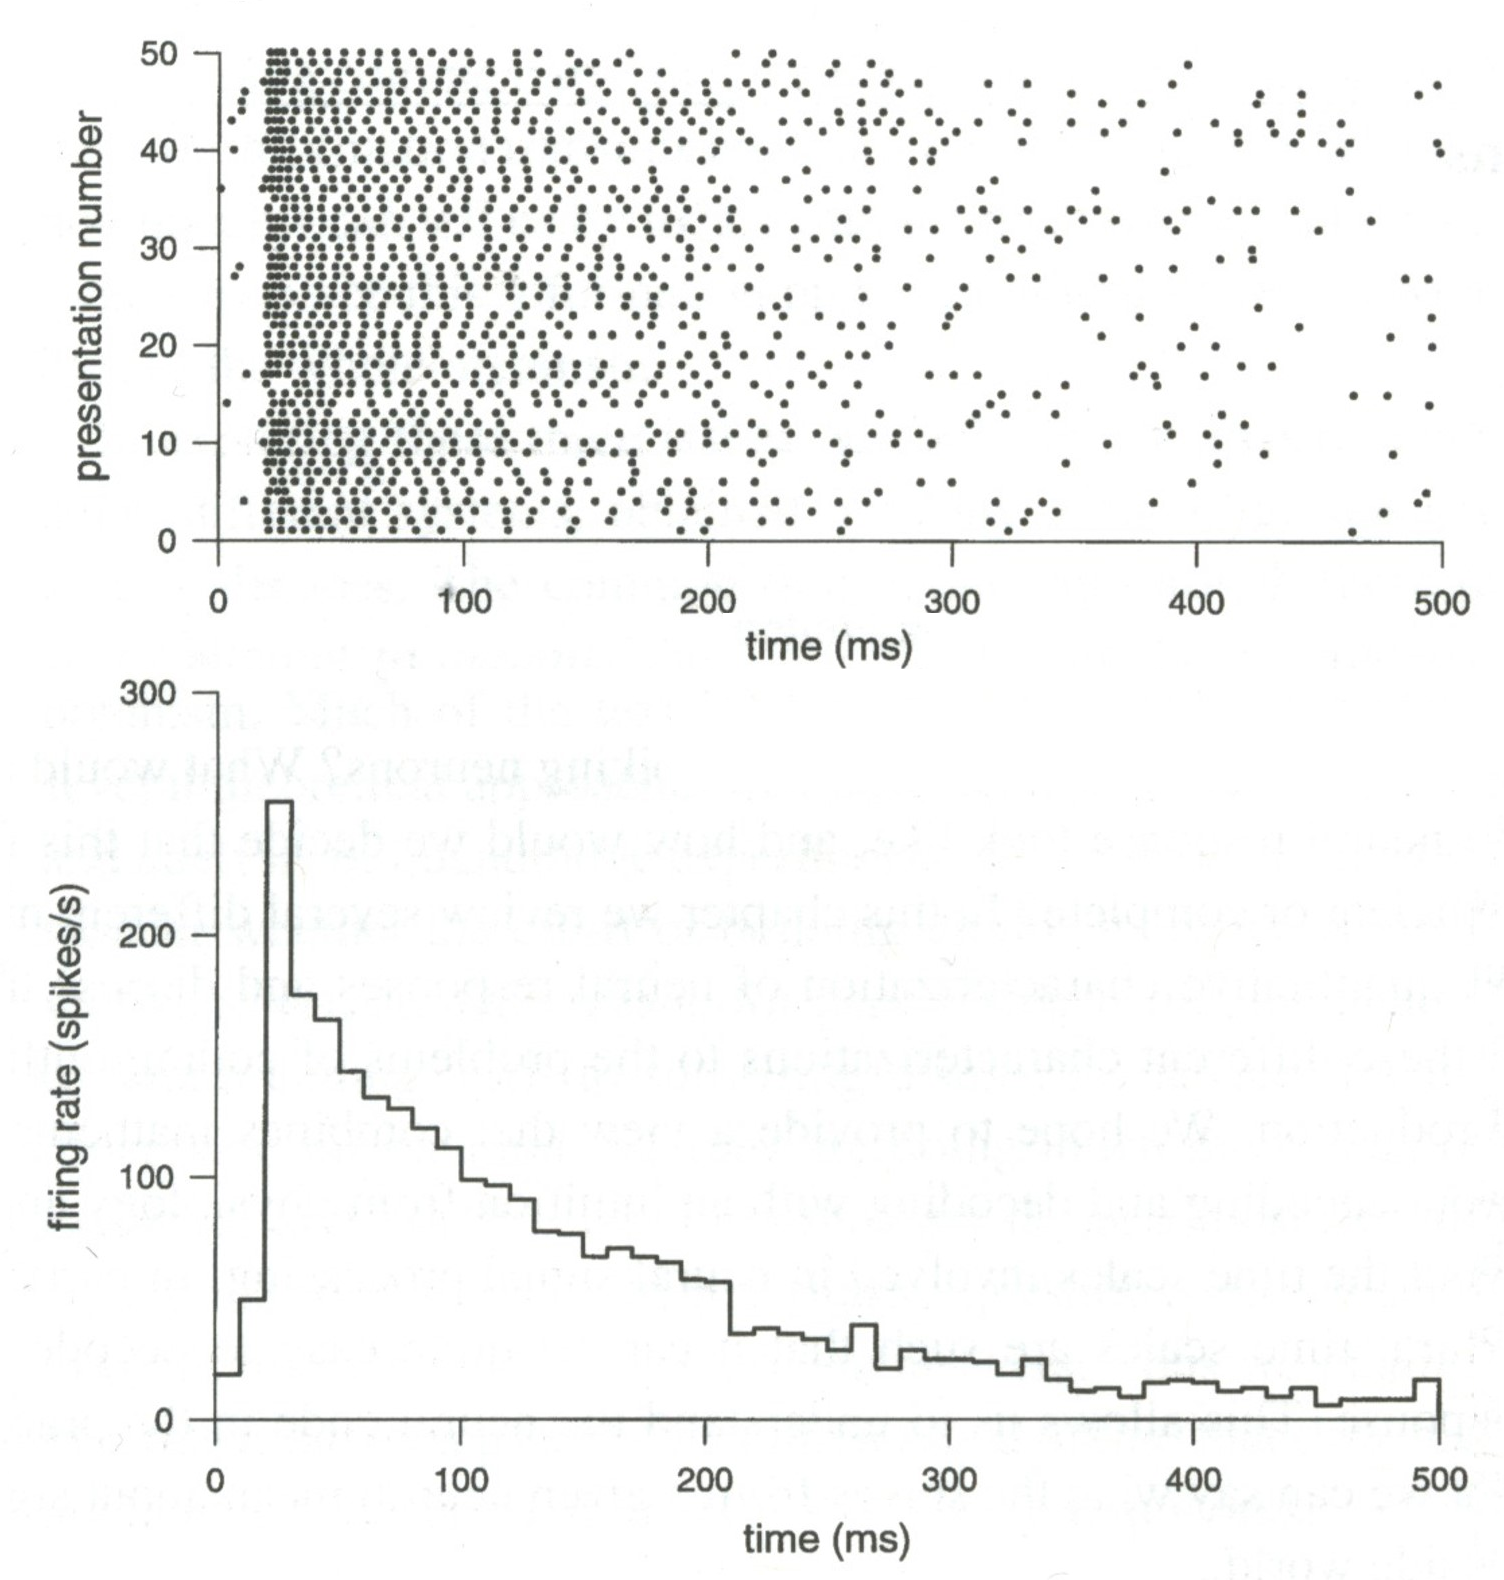
\includegraphics[scale=0.3]{8_2}
    \centering
\end{figure}
Generally, after after being stimulated, a neuron exhibits two different responses:
\begin{itemize}
    \item \textbf{Early response:} it occurs in the first \(50\,ms\) after the stimulus
          and includes the direct activation of the neuron.
    \item \textbf{Late (or delayed) response:} it occurs at least after \(50\,ms\) and up to
          \(400\,ms\), representing a reverberating response.
\end{itemize}
It can be said that the early response is definitely more reliable than the late
response, as the second one might be influenced by noise. A way to better focus
on the early response direct activation consists in chemically blocking the synapses.
\begin{figure}[H]
    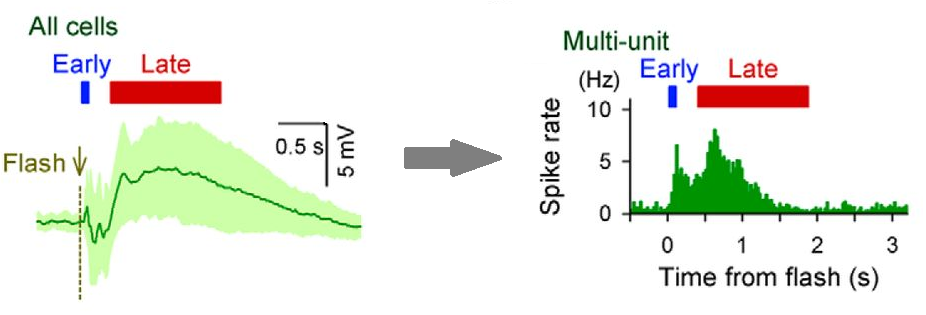
\includegraphics[scale=1.75]{8_3}
    \centering
\end{figure}
In addition, PST histograms might represent a valuable tool to individuate Major Burst
Leaders (MBLs), as they highlight the rapidity of a neuron to produce a response. In the
following picture a PSTH for each channel of an array of electrodes is represented,
according to the physical layout of the electrodes, and the MBLs are highlighted in red.
\begin{figure}[H]
    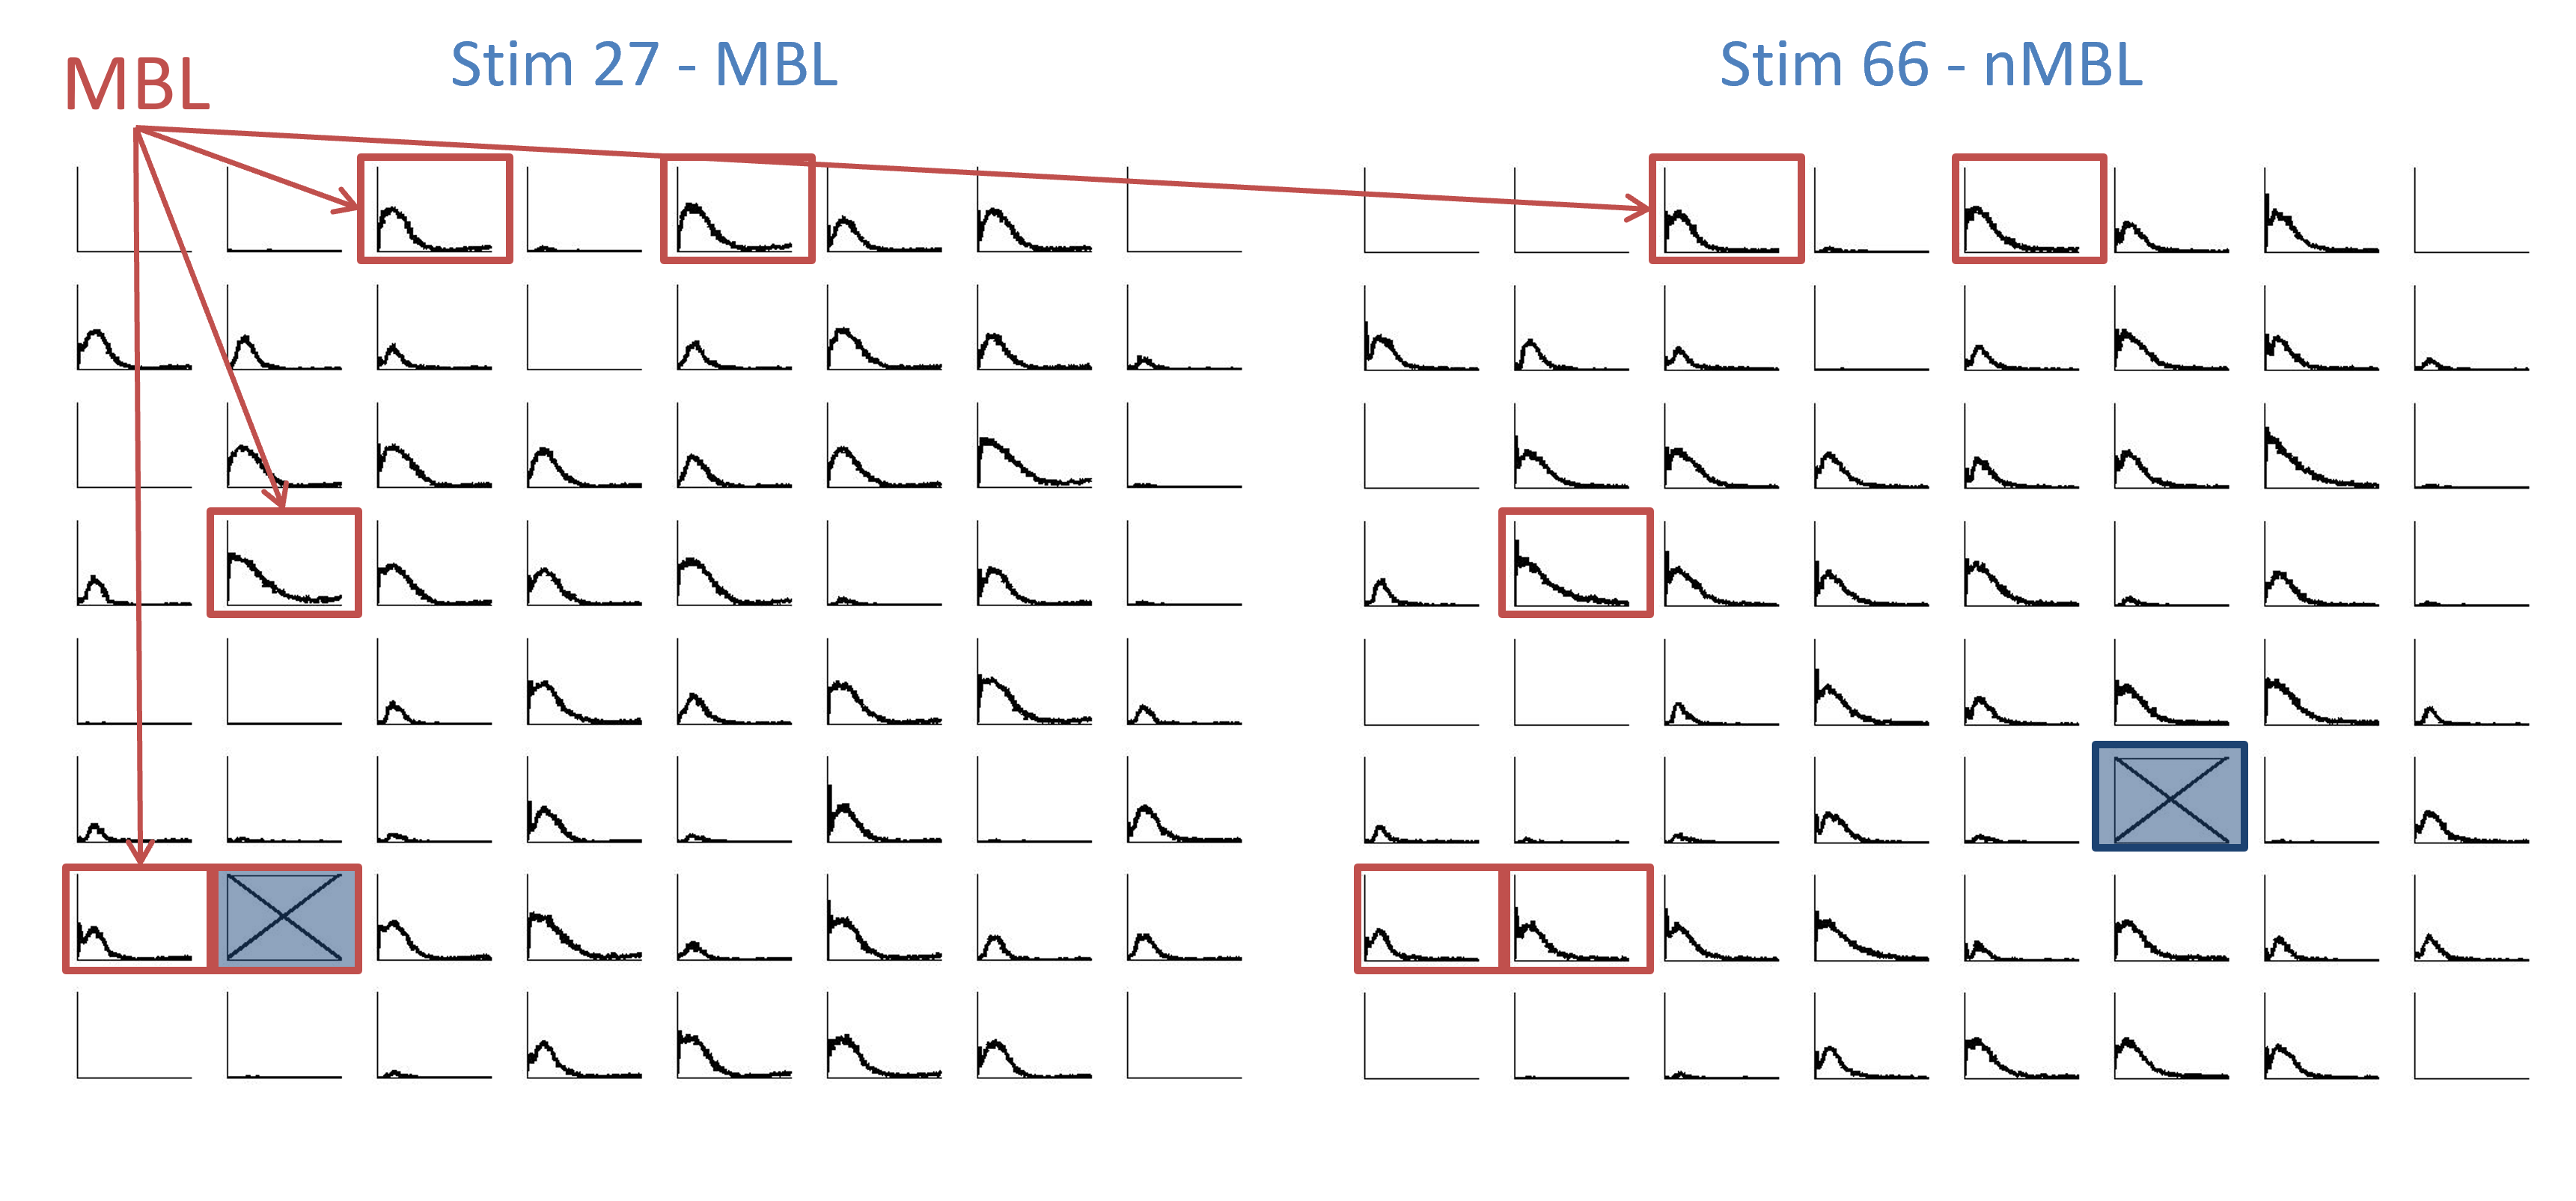
\includegraphics[scale=0.6]{8_4}
    \centering
\end{figure}